%% LaTeX2e class for student theses
%% sections/apendix.tex
%% 
%% Karlsruhe Institute of Technology
%% Institute for Program Structures and Data Organization
%% Chair for Software Design and Quality (SDQ)
%%
%% Dr.-Ing. Erik Burger
%% burger@kit.edu
%%
%% Version 1.3.5, 2020-06-26

\iflanguage{english}
{\chapter{Appendix}}    % english style
{\chapter{Anhang}}      % german style
\label{chap:appendix}


%\section{First Appendix Section}

%% -------------------
%% | Example content |
%% -------------------
%\label{sec:appendix:FirstSection}
		
\setcounter{figure}{0}
		
\begin{algorithm}[h]
  \caption{\textsc{CircleSetContour}}\label{alg:CircleSetContour}
  
  
  % Some settings
  \DontPrintSemicolon %dontprintsemicolon
  \SetFuncSty{textsc}
  \SetKwFor{ForAll}{forall}{do}
  
  
  % Declaration of data containers and functions
  \SetKwData{Q}{Q}
  \SetKwData{C}{C}
  \SetKwData{G}{G}
  \SetKwData{L}{L}
  \SetKwData{dist}{d}
  \SetKwData{pred}{pred}
  \SetKwFunction{queueDeleteMin}{deleteMin}
  \SetKwFunction{append}{append}
  \SetKwFunction{queueInsert}{insert}
  \SetKwFunction{queueDecreaseKey}{decreaseKey}
  \SetKwFunction{queueContains}{contains}
  \SetKwFunction{insertEdge}{addEdge}
  \SetKwFunction{queueContains}{contains}
  \SetKwFunction{location}{location}
  \SetKwFunction{angleBt}{angle}
  \SetKwFunction{angleToVec}{angleToVec}
  \SetKwFunction{vecToAngle}{vecToAngle}
  \SetKwFunction{intersect}{intersections}
  \SetKwFunction{neigh}{neighbors}
  \SetKwFunction{points}{pointsInRange}
  
  \SetKwRepeat{Do}{do}{while}
  
  % Algorithm interface
  \KwIn{Set \C of circles}
  \KwData{Graph $\G = (\C, \emptyset)$}
  \KwOut{List of contour sections $\C$ in order}
  
  % The algorithm
  \BlankLine
  \tcp{Generate graph}
  \ForAll{$(c_1,c_2) \in \C \times \C$}{
    \If{distance$(c_1, c_2) < c_1.radius + c_2.radius$}{
      \G.\insertEdge{$c_1, c_2$}
    }
  }
  
  \BlankLine
  \tcp{Find contour sections}
  $c_{max} \in \{c_i \in \C | \forall m \in \{1..|\C|\}: c_m.x + c_m.radius \leqslant c_i.x + c_i.radius\}$
  
  $c\leftarrow c_{max}$
  
  $\vec{p} \leftarrow \begin{pmatrix}
    1 \\
    0
  \end{pmatrix}$
  
  $\alpha \leftarrow 0$
  
  \Do{$c_{max} \neq c$}{
    \tcp{Find adjacent circle with intersection of smallest angle}
    $ \left(c_{next}, \beta \right) \leftarrow 
    \min_2{\left\{ 
      (n, \gamma)\ \middle\vert 
      \begin{array}{l}
        n \in \G.\neigh\left(c\right), \\
        \gamma  = 
          \min\left\{
            \angleBt{
              p, \intersect{n,c}
            }
          \right\}
      \end{array}
    \right\}} 
    $
  
    $\C.\append \left(
        \left(c , \alpha , \beta \right)
      \right)
    $
  
    \tcp{Calculate start direction vector of the next circle}
    $ \vec{p} \leftarrow \left( c.center + (\angleToVec(\beta) * c.radius ) - c_{next}.center\right)$
    
    $ c \leftarrow c_{next} $
    
    $  a \leftarrow \vecToAngle(\vec{p}) $
  
    }
  
    \tcp{Finish contour of last circle}
    $\C.\append \left( c_{max}, \alpha, 0 \right)$
  
\end{algorithm}
  
  

\begin{figure*}
  \begin{multicols}{2}
      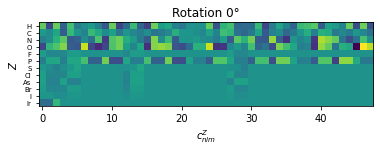
\includegraphics[width=\linewidth]{figures/regression/snap/rot0.png}\par 
      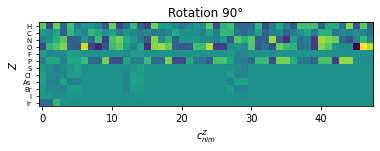
\includegraphics[width=\linewidth]{figures/regression/snap/rot90.png}\par 
  \end{multicols}
  \begin{multicols}{2}
      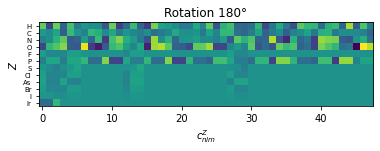
\includegraphics[width=\linewidth]{figures/regression/snap/rot180.png}\par
      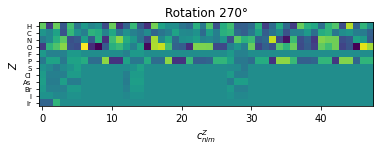
\includegraphics[width=\linewidth]{figures/regression/snap/rot270.png}\par
  \end{multicols}
  \caption{Visualization of SNAP descriptor output for the same element over different rotations.}
  \label{fig:snap_roation_out}
\end{figure*}



\begin{figure}
  \begin{subfigure}[t]{.155\textwidth}
    \centering
    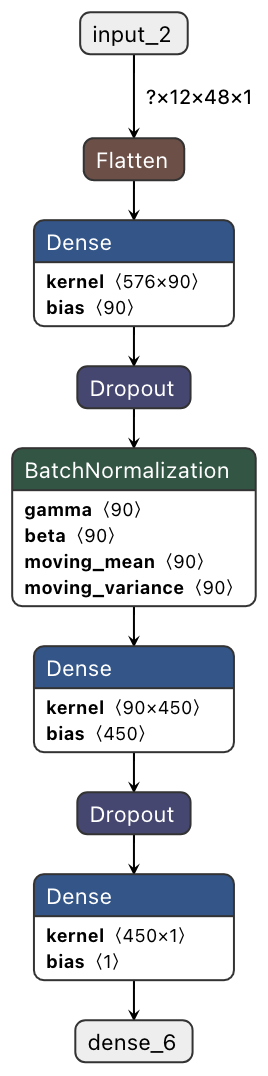
\includegraphics[width=\linewidth]{figures/regression/model_3-3.png}
    \caption{$n_{max}=3$, $l_{max}=3$}
  \end{subfigure}
  \hfill
  \begin{subfigure}[t]{.155\textwidth}
    \centering
    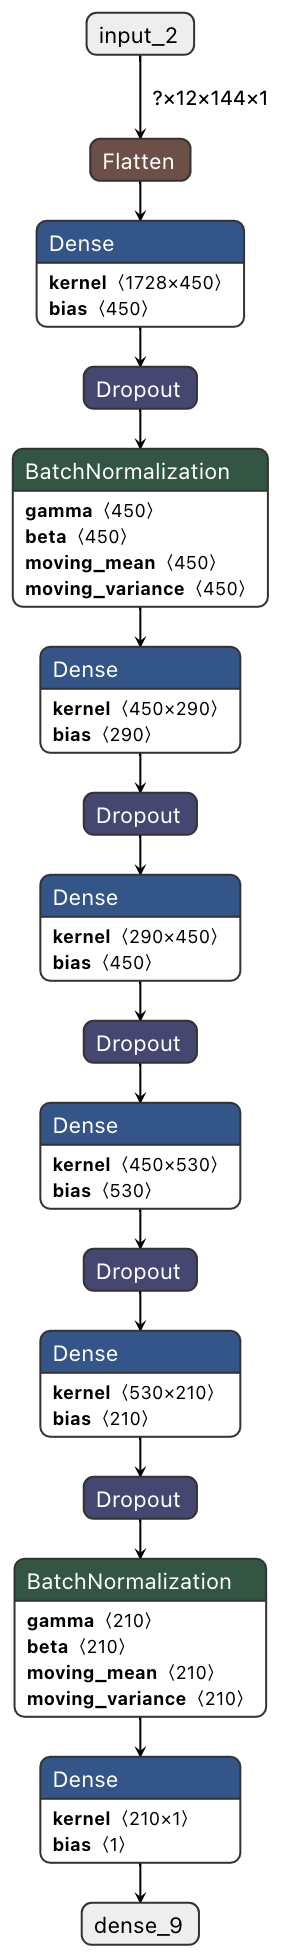
\includegraphics[width=\linewidth]{figures/regression/model_9-3.png}  
    \caption{$n_{max}=9$, $l_{max}=3$}
  \end{subfigure}
  \hfill
  \begin{subfigure}[t]{.155\textwidth}
    \centering
    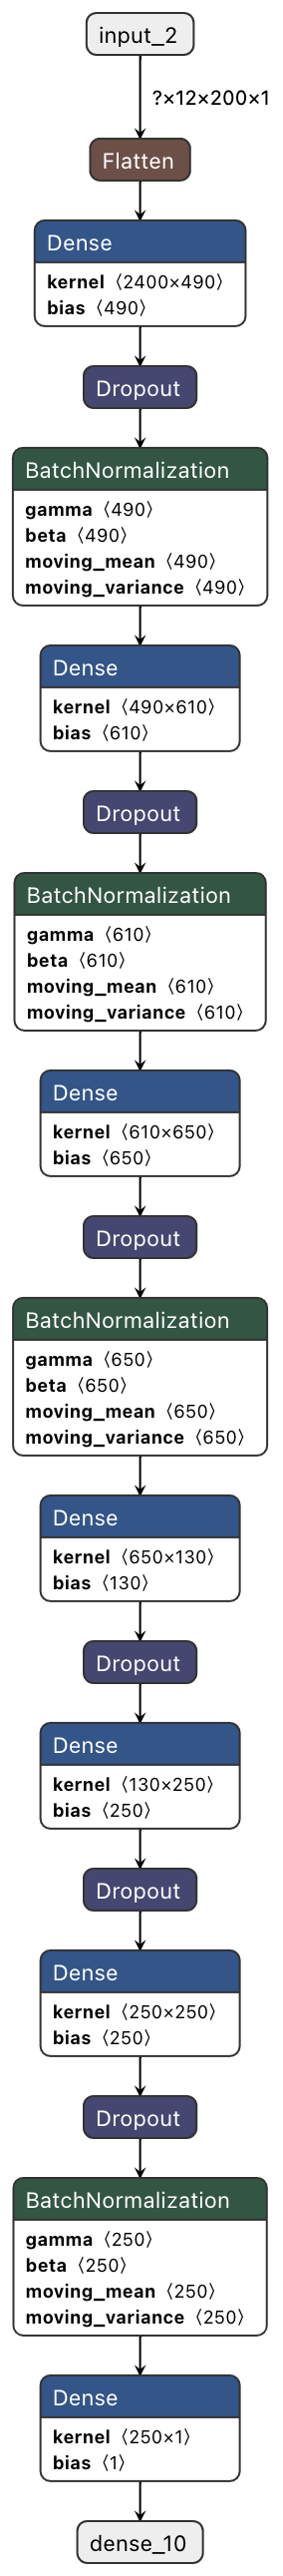
\includegraphics[width=\linewidth]{figures/regression/model_8-4.png}
    \caption{$n_{max}=8$, $l_{max}=4$}
  \end{subfigure}

  \caption{Network architecture for best performing SNAP regression networks.
  }
  \label{fig:transferlearn}
\end{figure}

\begin{figure}
  \begin{subfigure}[t]{.5\textwidth}
    \centering
    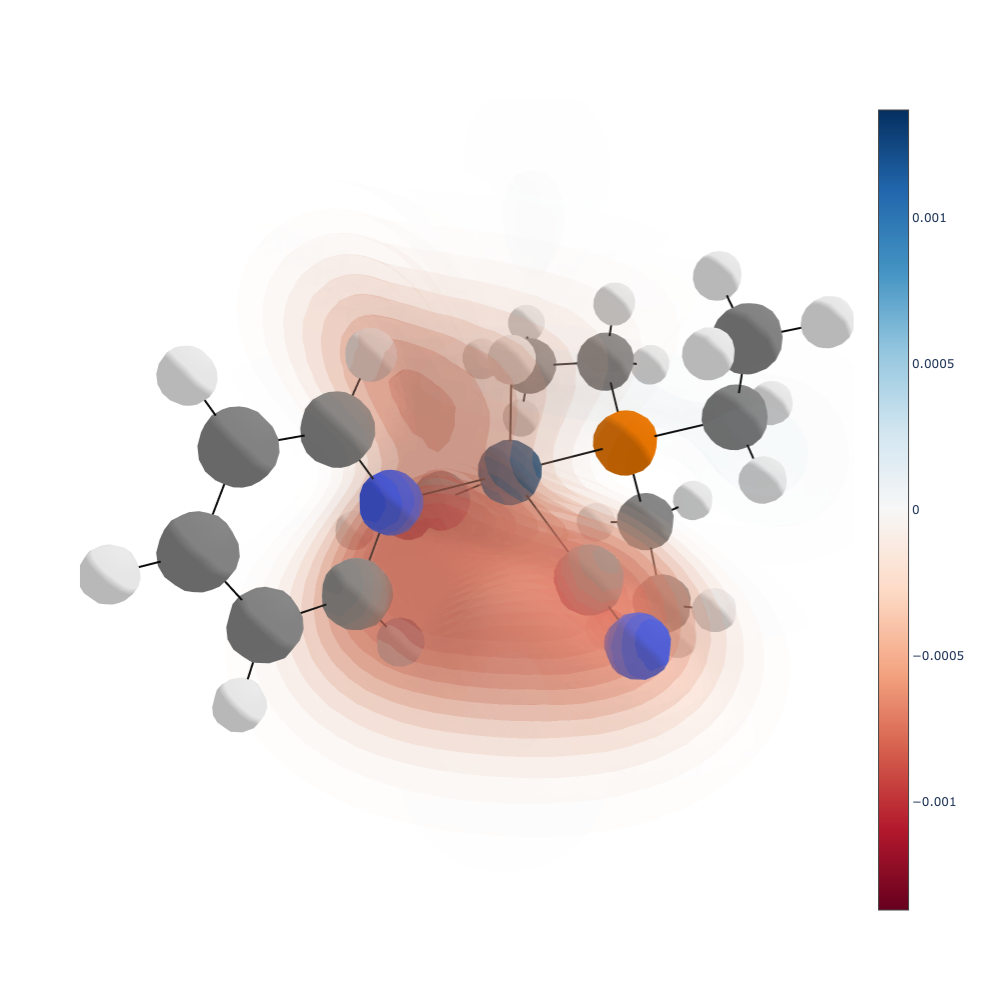
\includegraphics[width=\linewidth]{figures/evaluation/elem2-N.png}
  \end{subfigure}
  \hfill
  \begin{subfigure}[t]{.5\textwidth}
    \centering
    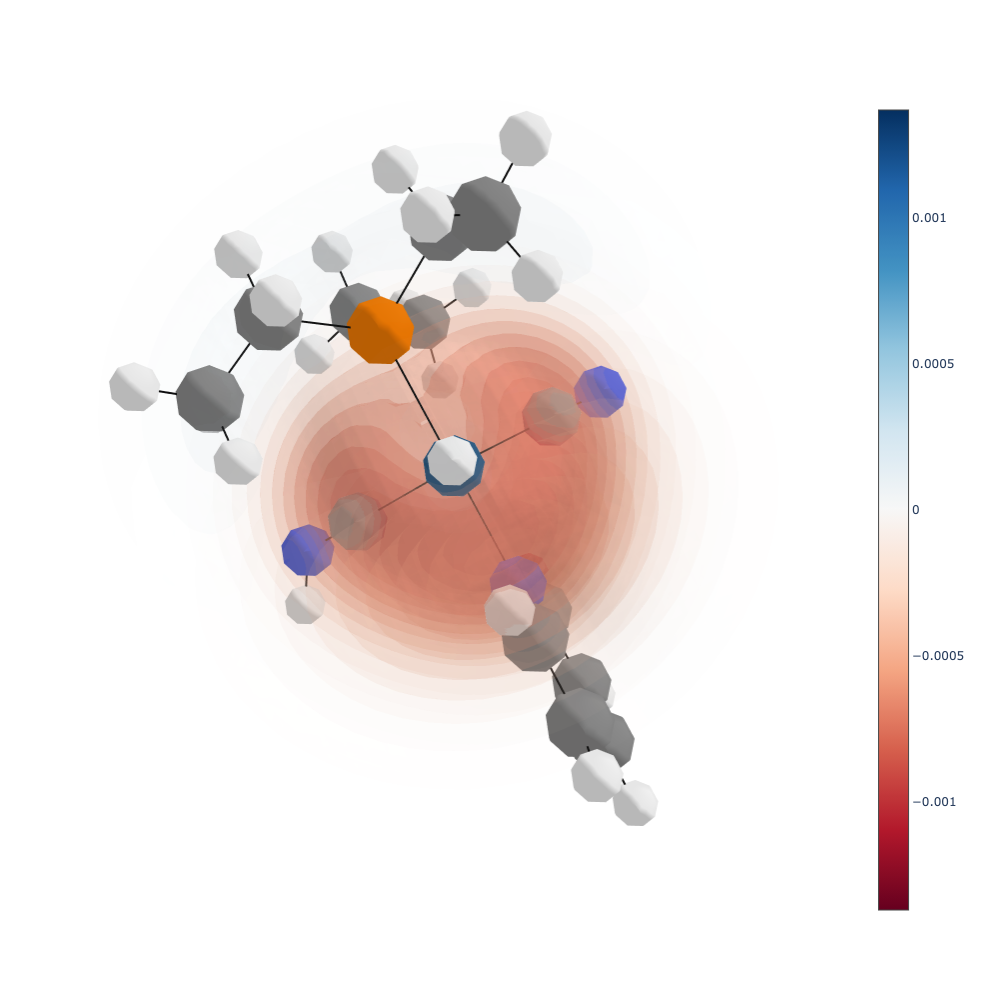
\includegraphics[width=\linewidth]{figures/evaluation/elem2-N-TOP.png}
  \end{subfigure}

  \medskip

  \begin{subfigure}[t]{.5\textwidth}
    \centering
    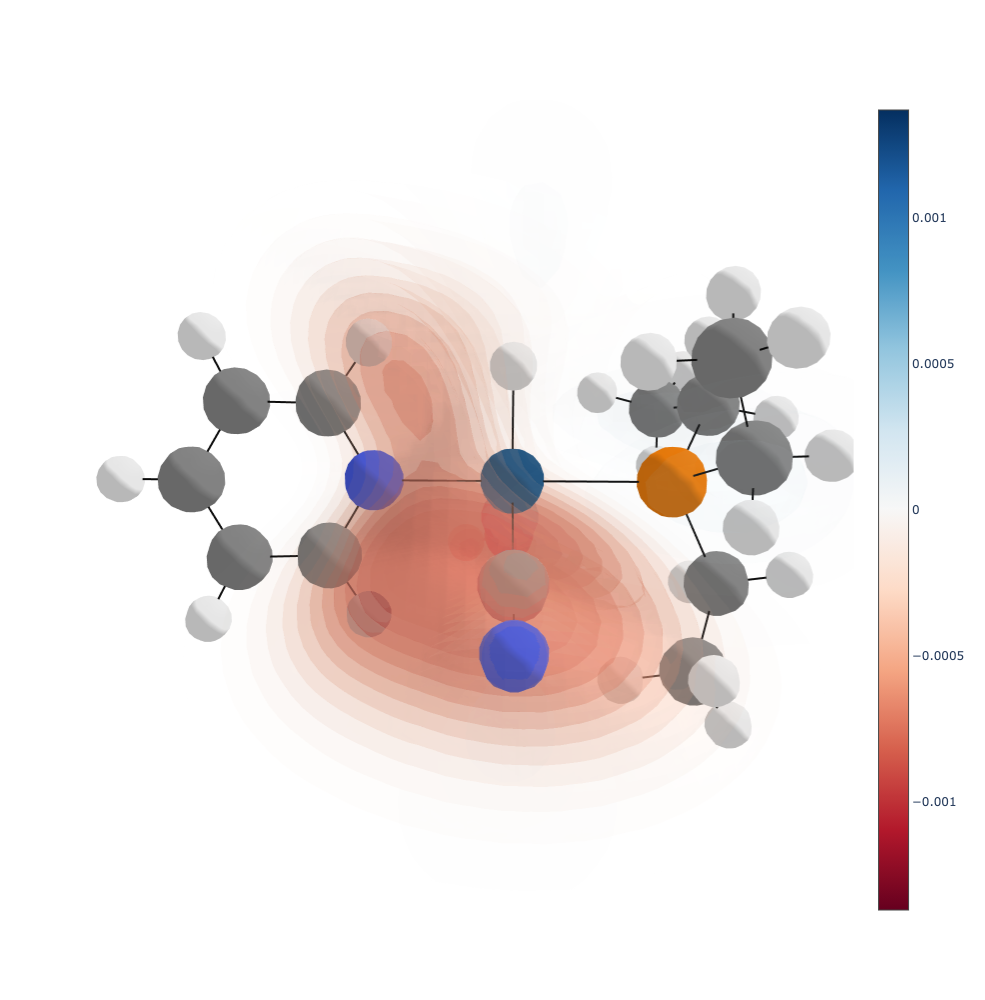
\includegraphics[width=\linewidth]{figures/evaluation/elem2-N-SIDE.png}
  \end{subfigure}
  \hfill
  \begin{subfigure}[t]{.5\textwidth}
    \centering
    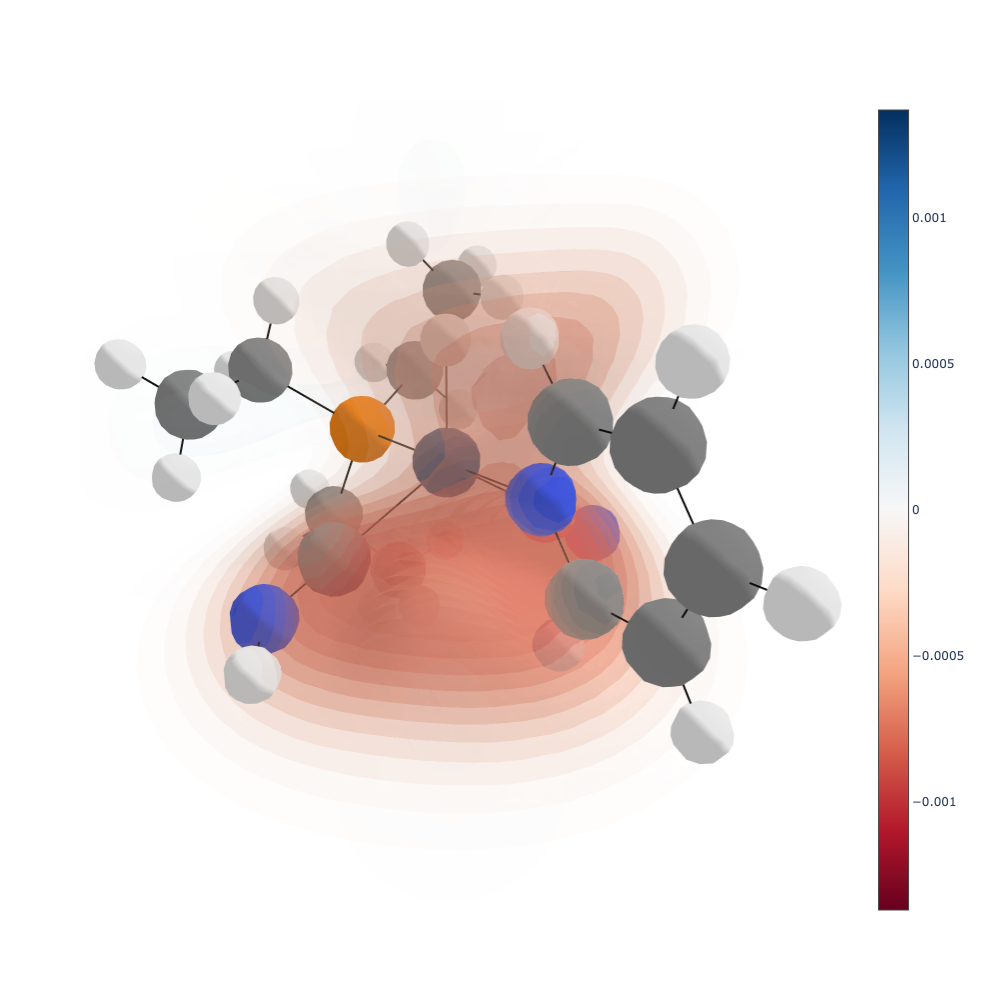
\includegraphics[width=\linewidth]{figures/evaluation/elem2-N-BACK.png}
  \end{subfigure}
  \caption{Gradient for nitrogen(blue) from multiple sides}
  \label{fig:gradient-sides}
\end{figure}


